\section{Evaluation}
\label{sec:eval}

We evaluate MiniMax-M2.7 against the strongest publicly deployed closed-weight frontier reasoning models---Claude Opus 4.6, Claude Sonnet 4.6~\citep{anthropic2025claude46}, GPT 5.4~\citep{openai2025gpt5}, and Gemini 3.1 Pro~\citep{google2025gemini31}---across three capability areas that mirror the design priorities of the M2 series: agentic coding, agentic cowork (search, multi-tool agents, and workspace operation), and reasoning \& knowledge. To make the within-series progression explicit, we additionally report scores for the previous public release, MiniMax-M2.5. Throughout, we deliberately favor benchmarks that exercise long-horizon, environment-grounded behavior over closed-form QA, since those are the regimes the M2 data pipelines and Forge RL system are explicitly built for.

\subsection{Evaluation Settings}

\noindent \textbf{Models and inference modes.} Each closed-weight baseline is evaluated in its strongest reasoning configuration: Claude Opus 4.6 and Claude Sonnet 4.6 with extended thinking, GPT 5.4 with high reasoning effort, and Gemini 3.1 Pro with high reasoning effort. M2.7 and M2.5 are evaluated with thinking enabled and the interleaved-thinking trajectory protocol described in \S\ref{sec:interleaved-thinking}. Unless otherwise noted, generation uses temperature 1.0 and top-p 0.95; on agentic benchmarks all models share the same scaffold and tool environment.

\noindent \textbf{Benchmarks.} We organize the reported benchmarks into five blocks:

\begin{itemize}
    \item \textbf{Software engineering and coding agent.} \emph{SWE-bench Pro}~\citep{swebenchpro2025} for industry-grade repository repair; \emph{SWE-bench Multilingual}~\citep{rashid2025swebenchmultilingual} for cross-language repository-level editing; \emph{Multi-SWE-bench}~\citep{multiswebench2025} for multi-repo task transfer; \emph{NL2Repo}, our internal natural-language-to-repository synthesis benchmark; \emph{Terminal-Bench 2.0}~\citep{merrill2026terminalbench} for terminal and system-operation tasks; and \emph{MLE Bench Lite}~\citep{chan2025mlebench} for autonomous machine-learning engineering, which we revisit as a self-evolution case study in \S\ref{sec:eval-case}.

    \item \textbf{Application development.} \emph{VIBE-Pro}, our internal end-to-end full-stack application development benchmark; and \emph{HyperTask}, an internal long-horizon ``vibe coding'' suite of $\sim$100 feature- or step-level requirements per task.

    \item \textbf{Cowork --- search and deep research.} \emph{BrowseComp}~\citep{wei2025browsecomp}, \emph{Wide Search}~\citep{liu2025widesearch}, and our internal \emph{RISE} benchmark for multi-step browsing under realistic web complexity.

    \item \textbf{Cowork --- agent, office, and workspace.} \emph{GDPval-AA}~\citep{patwardhan2025gdpvalevaluatingaimodel}, the Artificial-Analysis-judged subset of OpenAI's GDPval office-task suite; \emph{Toolathlon}~\citep{huang2025toolathlon} for heterogeneous tool use; \emph{MM Claw}, our internal multi-modal office-claw benchmark; \emph{MEWC v2}, an internal hard-task subset of 100 problems drawn from the Microsoft Excel World Championship pool; and \emph{Finance Modeling Pro}, an internal Excel-grounded financial-modeling suite scored by expert rubrics.

    \item \textbf{Reasoning and knowledge.} \emph{AIME 2026}~\citep{aime2026} for competition mathematics; \emph{GPQA-Diamond}~\citep{rein2024gpqa} for graduate-level science; \emph{SciCode}~\citep{tian2024scicode} for scientific code generation; \emph{IFBench}~\citep{pyatkin2025ifbench} for instruction following; \emph{AA-LCR} (Artificial Analysis Long-Context Reasoning) for retrieval-and-reasoning over long inputs; \emph{HLE}~\citep{phan2025humanity} (Humanity's Last Exam, no-tool subset) for frontier-difficulty open knowledge; and \emph{MMLU-Pro}~\citep{wang2024mmlu} for broad knowledge.
\end{itemize}

\noindent \textbf{Evaluation configurations.} \emph{SWE-bench Pro}, \emph{SWE-bench Multilingual}, \emph{Multi-SWE-bench}, and \emph{NL2Repo} are run on internal infrastructure with Claude Code as the unified scaffold (default system prompt overridden) for all models except GPT 5.4, which uses its native CodeX scaffold; results are averaged over 4 trials. \emph{Terminal-Bench 2.0} uses an 8 vCPU / 16\,GB sandbox with a 2\,hour wall-clock timeout, the Terminus-2 XML scaffold, and the verified 2.0 dataset (HuggingFace \path{zai-org/terminal-bench-2-verified}); 4 trials per model, baseline scores cited from official reports where not re-evaluated. \emph{MLE Bench Lite} runs each of the 22 competitions in a single-A30 sandbox for 24\,hours under our internal self-evolution scaffold (Bash + WebSearch); per-task scoring takes the best validation checkpoint and reports test-set medal rate; the final number is the mean of 3 independent 24-hour trials. \emph{VIBE-Pro} uses Claude Code as the verifier for both interaction logic and visual fidelity, end-to-end through a containerized deployment, 3 trials averaged. \emph{HyperTask}, \emph{MM Claw}, \emph{MEWC v2}, and \emph{Finance Modeling Pro} use expert-defined rubrics scored over 3 trials. \emph{BrowseComp}, \emph{Wide Search}, and \emph{RISE} share the \emph{WebExplorer}~\citep{liu2025webexplorer} agent framework, with light edits to the system prompt and tool descriptions; when token usage exceeds 30\,\% of the maximum context, all assistant replies and tool returns are dropped to keep the search alive. \emph{RISE} additionally enables a Playwright-based browser tool. \emph{GDPval-AA} is the Artificial Analysis re-evaluation on OpenAI's open GDPval dataset. \emph{AIME 2026}, \emph{GPQA-Diamond}, \emph{SciCode}, \emph{IFBench}, \emph{AA-LCR}, \emph{HLE}, and \emph{MMLU-Pro} are evaluated under the \emph{Artificial Analysis} Index v4.0 protocol with no tools and a single sample (pass@1).

\subsection{Main Results}

Table~\ref{tab:m2-main-results} reports M2.7 against four closed-weight frontier baselines (Claude Opus 4.6, Claude Sonnet 4.6, GPT 5.4, Gemini 3.1 Pro). The previous public M2 release (M2.5) is included as the within-series reference. The strongest score per row is \textbf{bolded}; ``--'' indicates that the model has not reported a score under our scaffold or has not yet released that benchmark at the time of writing.

\begin{table}[!t]
\scriptsize
\renewcommand{\arraystretch}{1.05}
\centering
\caption{\textbf{Performance of MiniMax-M2.7 versus closed-weight frontier baselines.} The MiniMax-M2.5 column gives the previous public release for within-series comparison.}
\setlength{\tabcolsep}{3.5pt}
\begin{tabular}{c|l|cc|cccc}
\toprule
& \multirow{2}{*}{\textbf{Benchmark}}
& \multicolumn{2}{c|}{\textbf{Ours}}
& \multicolumn{4}{c}{\textbf{Closed-weight frontier}} \\
\cmidrule(lr){3-4} \cmidrule(lr){5-8}
&
& \textbf{M2.7} & \textbf{M2.5}
& \makecell{\textbf{Opus} \\ \textbf{4.6}}
& \makecell{\textbf{Sonnet} \\ \textbf{4.6}}
& \makecell{\textbf{GPT} \\ \textbf{5.4}}
& \makecell{\textbf{Gemini} \\ \textbf{3.1 Pro}} \\
\midrule
\multirow{6}{*}{\rotatebox[origin=c]{90}{\shortstack{\textbf{Coding} \\ \textbf{Agent}}}}
 & SWE-bench Pro          & 56.2 & 55.4 & 57.3 & 57.2 & \textbf{57.7} & 54.2 \\
 & SWE-bench Multilingual & 76.5 & 74.1 & \textbf{77.8} & 75.9 & 70.5 & --   \\
 & Multi-SWE-bench        & \textbf{52.7} & 51.3 & 50.3 & 51.0 & 49.0 & --   \\
 & NL2Repo                & 39.8 & 26.6 & 43.7 & 43.3 & \textbf{46.8} & 35.9 \\
 & Terminal-Bench 2.0     & 57.0 & 51.7 & 65.4 & 59.1 & \textbf{75.1} & 68.5 \\
 & MLE Bench Lite         & 66.6 & 51.5 & \textbf{75.7} & 72.7 & 71.2 & 66.6 \\
\cmidrule(lr){2-8}
\multirow{2}{*}{\rotatebox[origin=c]{90}{\shortstack{\textbf{App} \\ \textbf{Dev}}}}
 & VIBE-Pro               & 55.6 & 54.2 & 55.6 & \textbf{56.1} & --   & 41.0 \\
 & HyperTask              & 67.6 & 59.4 & \textbf{75.7} & 74.1 & --   & 50.9 \\
\cmidrule(lr){2-8}
\multirow{3}{*}{\rotatebox[origin=c]{90}{\textbf{Search}}}
 & BrowseComp             & 77.8 & 76.3 & 84.0 & 74.7 & 82.7 & \textbf{85.9} \\
 & Wide Search            & 75.2 & 70.3 & \textbf{79.4} & 75.8 & 77.9 & --   \\
 & RISE                   & 64.3 & 50.2 & \textbf{68.5} & 58.8 & 63.3 & --   \\
\cmidrule(lr){2-8}
\multirow{5}{*}{\rotatebox[origin=c]{90}{\shortstack{\textbf{Office} \\ \textbf{\& Tools}}}}
 & GDPval-AA              & 50.0 & 35.0 & 55.0 & 57.0 & \textbf{58.0} & 41.0 \\
 & Toolathlon             & 46.3 & 38.3 & 47.2 & 44.8 & \textbf{54.6} & 48.8 \\
 & MM Claw                & 62.7 & 57.6 & \textbf{75.4} & 64.2 & 73.6 & 61.8 \\
 & MEWC v2                & 63.3 & 49.8 & 62.0 & \textbf{77.2} & 76.5 & 42.2 \\
 & Finance Modeling Pro   & 57.0 & 33.8 & 69.0 & 66.2 & \textbf{75.3} & 35.6 \\
\cmidrule(lr){2-8}
\multirow{7}{*}{\rotatebox[origin=c]{90}{\shortstack{\textbf{Reasoning} \\ \textbf{\& Knowledge}}}}
 & AIME 2026              & 94.2 & 87.2 & 92.5 & 92.7 & \textbf{97.0} & 88.7 \\
 & GPQA-Diamond           & 89.8 & 85.2 & 89.6 & 87.5 & 92.0 & \textbf{94.1} \\
 & SciCode                & 47.0 & 43.0 & 51.9 & 46.8 & 56.6 & \textbf{58.9} \\
 & IFBench                & 76.0 & 72.0 & 53.1 & 56.6 & 73.9 & \textbf{77.1} \\
 & AA-LCR                 & 72.0 & 65.0 & 70.7 & 70.7 & \textbf{74.0} & 72.7 \\
 & HLE                    & 28.0 & 19.0 & 36.7 & 30.0 & 41.6 & \textbf{44.7} \\
 & MMLU-Pro               & 81.8 & 85.2 & 89.1 & 87.3 & 87.5 & \textbf{91.2} \\
\bottomrule
\end{tabular}
\label{tab:m2-main-results}
\end{table}

\noindent \textbf{Software engineering and coding agent.} M2.7 is broadly competitive across the agentic-coding suite. It scores 56.2 on \emph{SWE-bench Pro}, 76.5 on \emph{SWE-bench Multilingual}, takes the top score among compared models on \emph{Multi-SWE-bench} at 52.7, and reaches 57.0 on \emph{Terminal-Bench 2.0}. On \emph{NL2Repo} M2.7 reaches 39.8, a 13-point jump from M2.5 (26.6) that reflects the new full-stack repository data introduced in \S\ref{sec:agentic-coding-data}. On \emph{MLE Bench Lite} M2.7 reaches a 66.6\,\% medal rate, a 15-point absolute jump over M2.5; we discuss this case in detail in \S\ref{sec:eval-case}.

\noindent \textbf{Application development.} On \emph{VIBE-Pro} M2.7 reaches 55.6, on par with the leading closed-weight baselines. On the harder long-horizon \emph{HyperTask} suite, M2.7 reaches 67.6, an 8-point improvement over M2.5. Application development is one of the cleanest domains for the M2 design thesis: with $\sim$10\,B activated parameters, the AppDev-targeted training data and Agent-as-a-Verifier reward (\S\ref{sec:agentic-coding-data}) close most of the gap to frontier models that activate an order of magnitude more parameters per token.

\noindent \textbf{Cowork --- search and deep research.} On the open-web search-and-synthesize triad, M2.7 reaches 77.8 on \emph{BrowseComp}, 75.2 on \emph{Wide Search}, and 64.3 on our internal \emph{RISE} benchmark (designed to require non-trivial multi-step browsing and cross-source corroboration with a Playwright browser tool). RISE also marks the largest within-series gain in this block, climbing 14 points from M2.5 (50.2). M2.7 is most competitive on tasks demanding longer planning horizons and richer web interaction, consistent with the verifier-grounded data pipeline used to construct our deep-search training corpus (\S\ref{sec:agentic-cowork-data}) and the persistent reasoning state of interleaved thinking across many turns (\S\ref{sec:interleaved-thinking}).

\noindent \textbf{Cowork --- agent, office, and workspace.} On heterogeneous tool-use benchmarks, M2.7 reaches 50.0 on \emph{GDPval-AA} and 46.3 on \emph{Toolathlon}. On Excel-grounded operation, M2.7 reaches 63.3 on \emph{MEWC v2} and 57.0 on \emph{Finance Modeling Pro}; on \emph{MM Claw} M2.7 reaches 62.7. This block shows the largest within-series headroom of any capability area in the M2 series, with substantial M2.5\,$\to$\,M2.7 gains on Excel-grounded benchmarks (\emph{MEWC v2} $+13.5$, \emph{Finance Modeling Pro} $+23.2$) and on \emph{GDPval-AA} ($+15.0$).

\noindent \textbf{Reasoning and knowledge.} M2.7 is competitive on the reasoning-heavy benchmarks where evaluation reduces to a single sample without tools. M2.7 scores 94.2 on \emph{AIME 2026}, 89.8 on \emph{GPQA-Diamond}, 76.0 on \emph{IFBench}, and 72.0 on \emph{AA-LCR}, placing it in the frontier band on each. The \emph{IFBench} result in particular reflects the multi-domain RL strategy and rubric-based response filtering described in \S\ref{sec:reasoning-data} and \S\ref{sec:rl}. On the broader knowledge benchmarks, M2.7 reaches 81.8 on \emph{MMLU-Pro}, 47.0 on \emph{SciCode}, and 28.0 on \emph{HLE}.

\noindent \textbf{Within-series progression.} To complement the cross-model snapshot of Table~\ref{tab:m2-main-results}, Figure~\ref{fig:m2-progression} traces the trajectory of the M2 series itself from the original M2 release through M2.5 to the current M2.7, restricted to the eleven benchmarks for which all three checkpoints have been evaluated under our scaffold. Two patterns stand out. First, every benchmark in this set improves across the three checkpoints, with absolute gains ranging from $+11$ points (AA-LCR, GPQA-Diamond) to $+33.8$ points (BrowseComp). Second, the size of the gain tracks the data-pipeline investments described in \S\ref{sec:post-training-data}: the benchmarks where the M2.5 / M2.7 corpora introduced new task families---deep search (BrowseComp $+33.8$, Wide Search $+12.9$), tool use (Toolathlon $+27.5$, GDPval-AA $+16.0$), and autonomous ML engineering (MLE Bench Lite $+26.6$)---show the steepest jumps, while benchmarks the original M2 was already strong on (SWE-bench Multilingual, Multi-SWE-bench) progress more incrementally. Reasoning benchmarks (AIME 2025 $+16.0$, GPQA-Diamond $+11.8$, AA-LCR $+11.0$) follow a steadier curve consistent with the multi-axis scaling of the reasoning data pipeline. Taken together, the figure indicates that each of the three contribution axes of the M2 series---agentic data, the Forge RL system (\S\ref{sec:rl}), and self-evolution (\S\ref{sec:self-evolution})---translates into a stable improvement trajectory at every release rather than concentrating in any single checkpoint.

\begin{figure*}[!t]
\centering
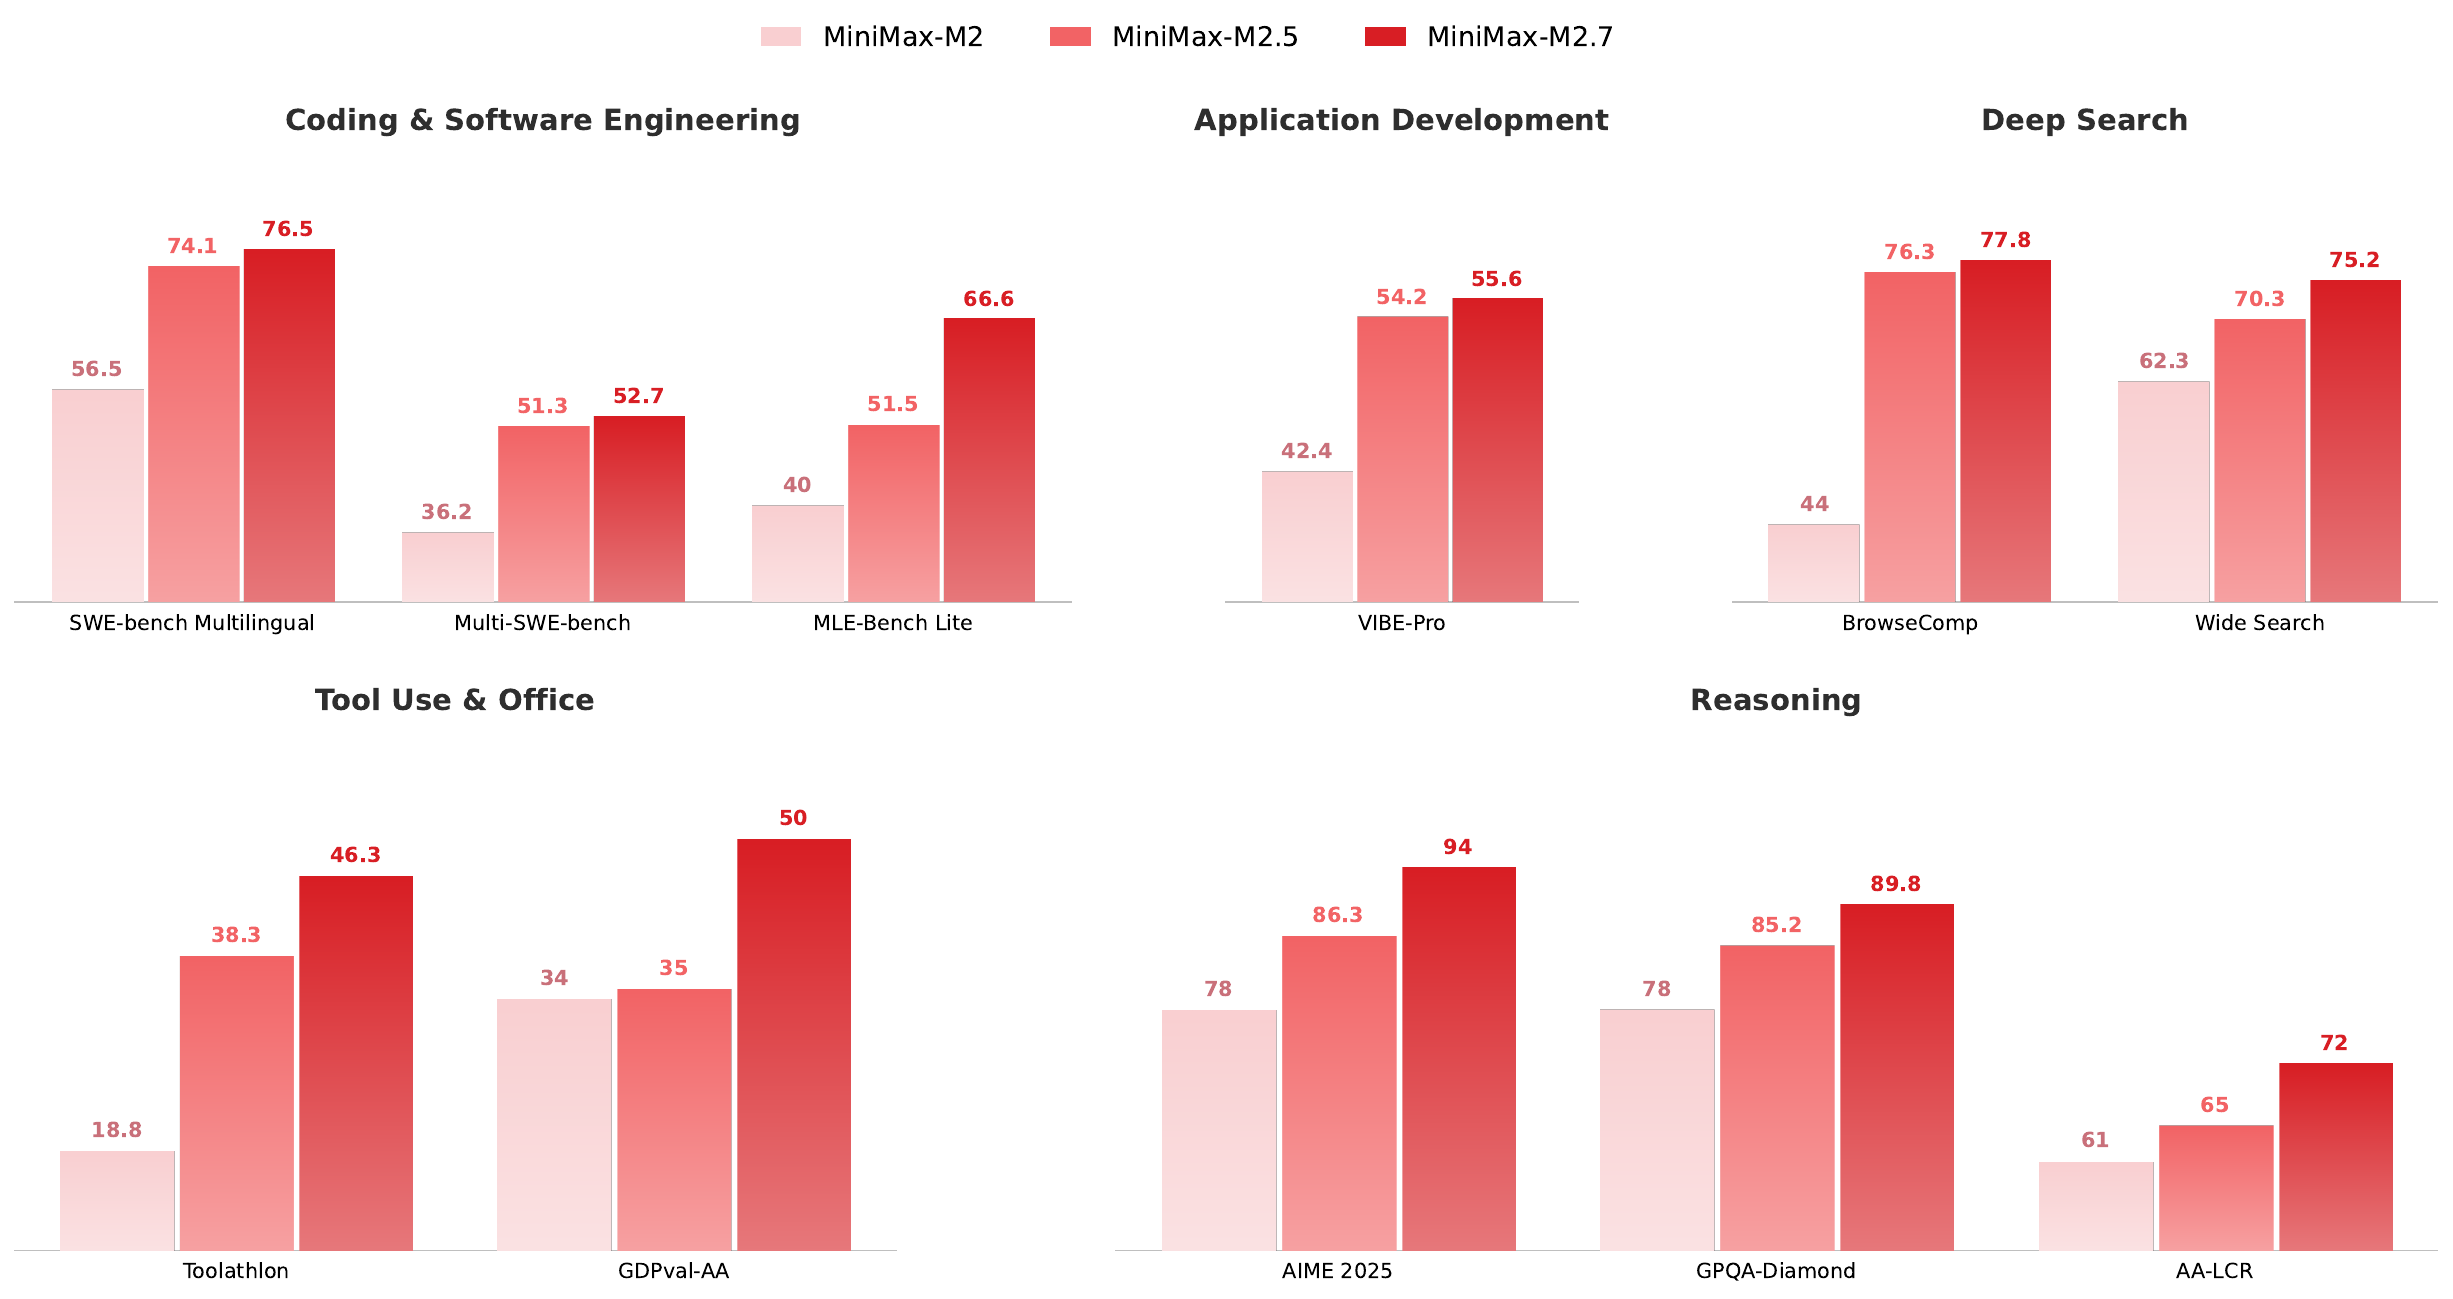
\includegraphics[width=\textwidth]{figures_new/m2_progression_optionA_v3.pdf}
\caption{\textbf{Capability progression of the MiniMax-M2 series across eleven benchmarks.} Each panel groups benchmarks by capability area, and within each benchmark the three bars correspond to the original M2 release, M2.5, and the current M2.7. AIME numbers in this figure refer to AIME 2025, the only AIME edition reported for all three checkpoints; the BrowseComp number for M2 is the Hugging Face official score. All eleven benchmarks improve across the three checkpoints, with the largest gains concentrated in the agentic deep-search, tool-use, and autonomous ML-engineering domains where the M2.5 / M2.7 data pipelines added new task families.}
\label{fig:m2-progression}
\end{figure*}

\subsection{Case Study: Self-Evolution on MLE Bench Lite}
\label{sec:eval-case}

\noindent The MLE Bench Lite result in Table~\ref{tab:m2-main-results} is the most direct evidence for the self-evolution capability whose system design is described in \Cref{sec:self-evolution}. The underlying driver is M2.7's strength in Machine Learning Engineering (MLE): on OpenAI's \emph{MLE Bench Lite}~\citep{chan2025mlebench}, M2.7 ties Gemini 3.1 Pro, demonstrating the frontier-level ability required to independently orchestrate ML pipelines and modify its own training scaffolds.

\noindent To test this capability under a controlled setting, we evaluated M2.7 as an independent ML engineer across 22 competitions from \emph{MLE Bench Lite}. While computationally lightweight, these tasks cover all stages of a standard ML workflow.

\noindent To guide the model, we implemented a simple autonomous harness driven by short-term memory and self-feedback, with no human-written code in the harness itself. After completing an iteration, the agent documents a memory file and performs rigorous self-criticism. This self-reflective critique establishes explicit optimization directions for subsequent runs, allowing the model to build upon an accumulated feedback chain.

\noindent We executed three independent trials, allowing 24\,hours of iterative evolution per run. As illustrated in Figure~\ref{fig:mle-medal-rate}, M2.7 demonstrated clear cumulative improvement, steadily increasing its medal rate over time. The best run yielded 9 gold medals, 5 silver medals, and 1 bronze medal. Averaging a 66.6\% medal rate across trials, M2.7 ties Gemini 3.1 Pro, demonstrating its capacity to autonomously navigate and optimize complex, end-to-end ML pipelines.

\noindent We highlight this case not just for the numerical outcome but for the qualitative observation that M2.7 willingly debugs its own training scaffold, modifies configuration files, and iterates over hundreds of rounds---behaviors that close the \emph{mini-activations $\to$ max real-world intelligence} loop the M2 series is designed around.

\begin{figure}[h]
\centering
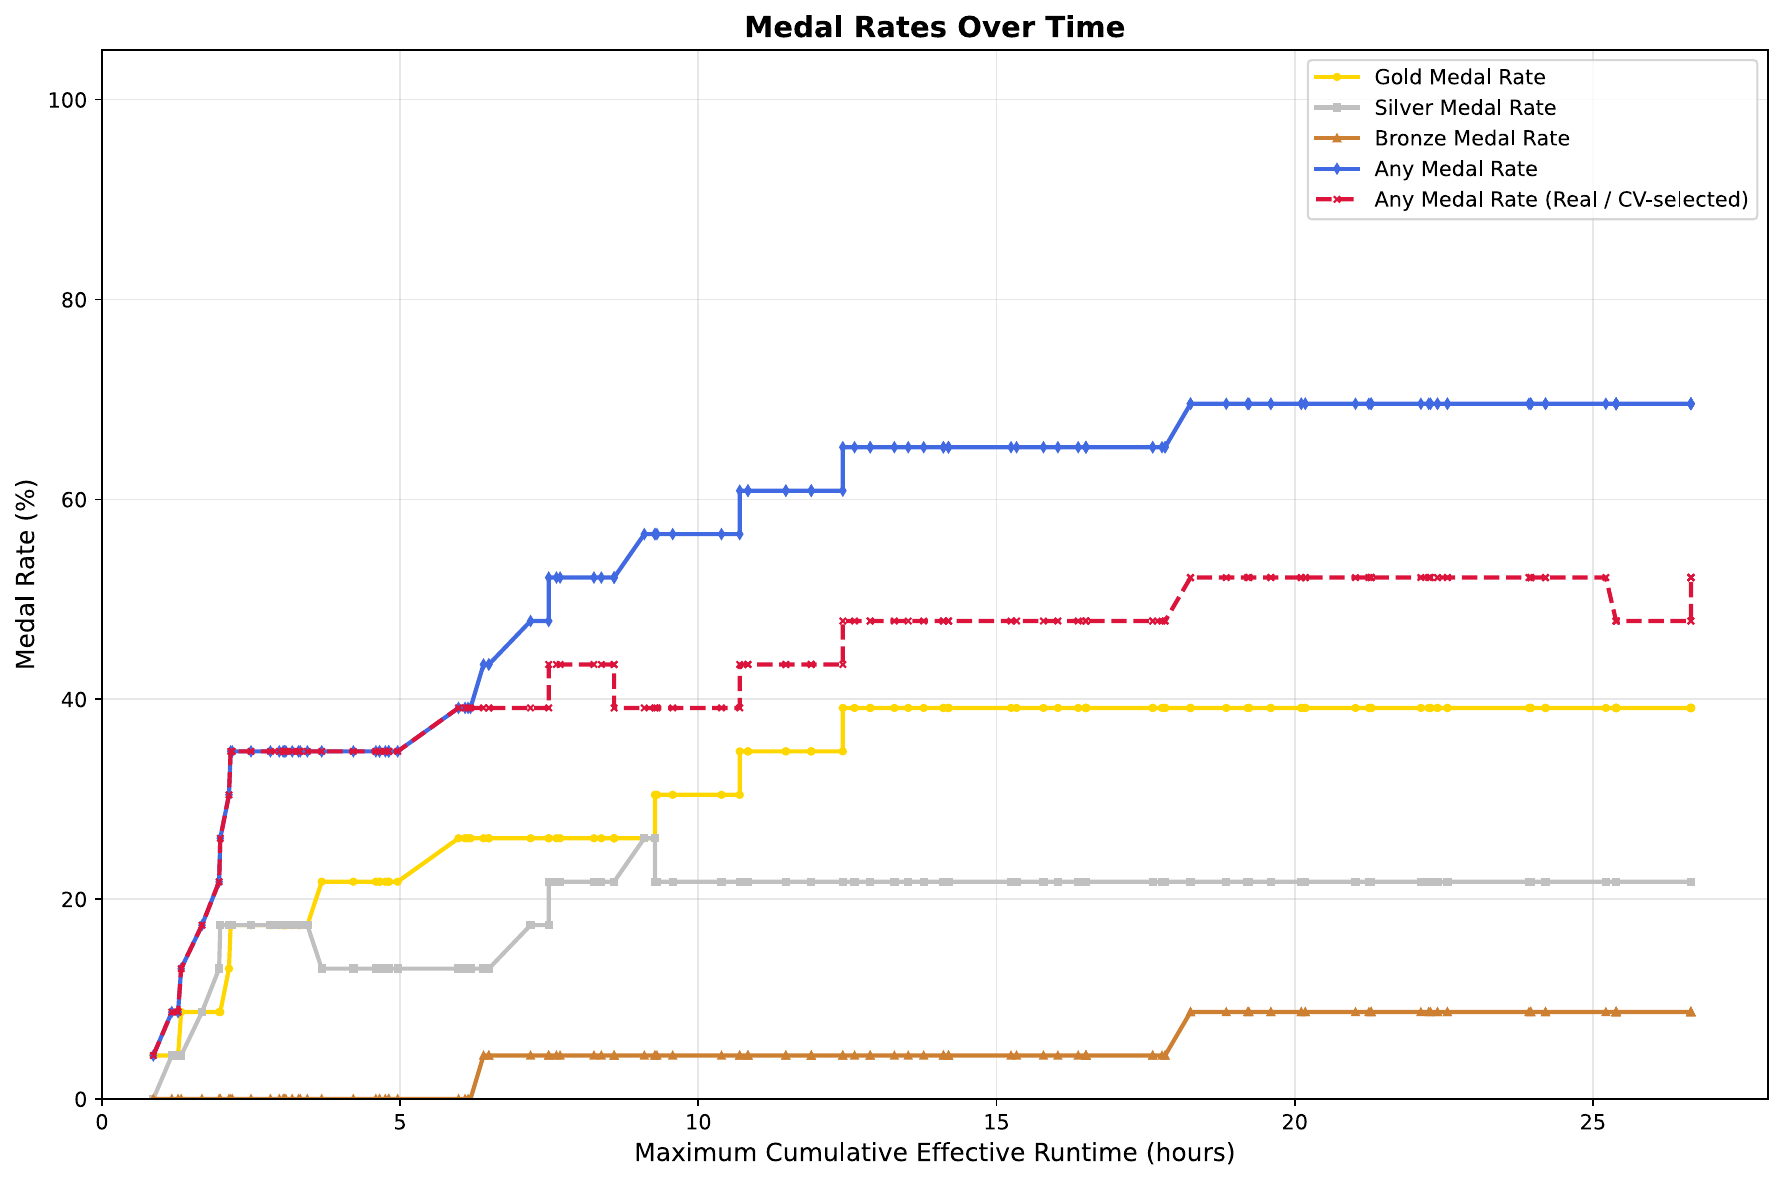
\includegraphics[width=0.74\textwidth]{figures_new/mle_medal_rate.pdf}
\caption{Medal rate of M2.7 on \emph{MLE Bench Lite} across iterative trials.}
\label{fig:mle-medal-rate}
\end{figure}
